\subsection{Motivation and State of the Field}

The integration of robotics and artificial intelligence into healthcare is advancing rapidly, driven by challenges such as aging populations, rising healthcare costs, and medical staff shortages. Researchers have developed various robotic solutions, including telepresence robots for remote consultations, autonomous robots for logistics, and socially assistive robots (SARs) for patient engagement. While each type has proven useful, they often function in isolation, addressing only part of patients' and clinicians' overall needs. The goal is to show that although the components for such a system already exist, combining them into a single, user-friendly, and autonomous platform remains an underexplored area with high potential, especially for improving healthcare accessibility in regions like Oman.

Telepresence robots, often described as a mobile screen, are widely used for remote medical consultations. Systems such as InTouch Health RP-VITA and the VGo robot have been used successfully in "telestroke" care, allowing neurologists to assess patients remotely, reduce diagnosis time, and improve outcomes \cite{garingo2016}. These systems support remote rounds, specialist consultations, and family visits, cutting travel costs and reducing infection risks. However, studies also note several drawbacks. A review by Kristoffersson et al. found that telepresence robots, though functional, often feel impersonal and difficult to control \cite{kristoffersson2013}. Clinicians report high cognitive load when navigating cluttered hospital spaces. Patients, especially the elderly and children, also find these robots less engaging than in-person visits due to limited physical embodiment and lack of expressive cues \cite{sabanovic2013}. This "presence gap" limits their effectiveness beyond basic video conferencing, reducing their ability to offer comfort and reassurance during care.

This literature review builds a comprehensive case for an integrated, autonomous healthcare robotics platform. It begins by examining success stories from consumer and industrial robotics, demonstrating that autonomous navigation technology has reached maturity and widespread adoption. The review then analyzes healthcare-specific applications, including telepresence, socially assistive robots, and hospital logistics systems, alongside their underlying technical components such as navigation systems, mobile platforms, conversational AI, and user interfaces. By systematically evaluating these technologies and their implementations, this survey identifies a critical research gap: the absence of a unified system that synthesizes clinical telepresence, social interaction, and autonomous mobility into a single platform.

\subsubsection{Success Stories: Consumer, Industrial, and Quadruped Robotics}

\begin{enumerate}[leftmargin=*]
    \item \textbf{Consumer Market: The Robotic Vacuum Revolution.}\newline
    The most successful deployment of autonomous mobile robots to the general public has been robotic vacuum cleaners, which dominate the consumer robotics market without serious competition from traditional cleaning methods. The global robotic vacuum cleaner market has experienced explosive growth, with projections indicating expansion from \$9.07 billion in 2024 to \$31.79 billion by 2033, representing a compound annual growth rate (CAGR) of 16.97\% \cite{imarc2024}. Global shipments reached 15.35 million units in the first half of recent years, demonstrating a 33\% year-over-year growth \cite{scmp2024}.

\begin{figure}[H]
\centering
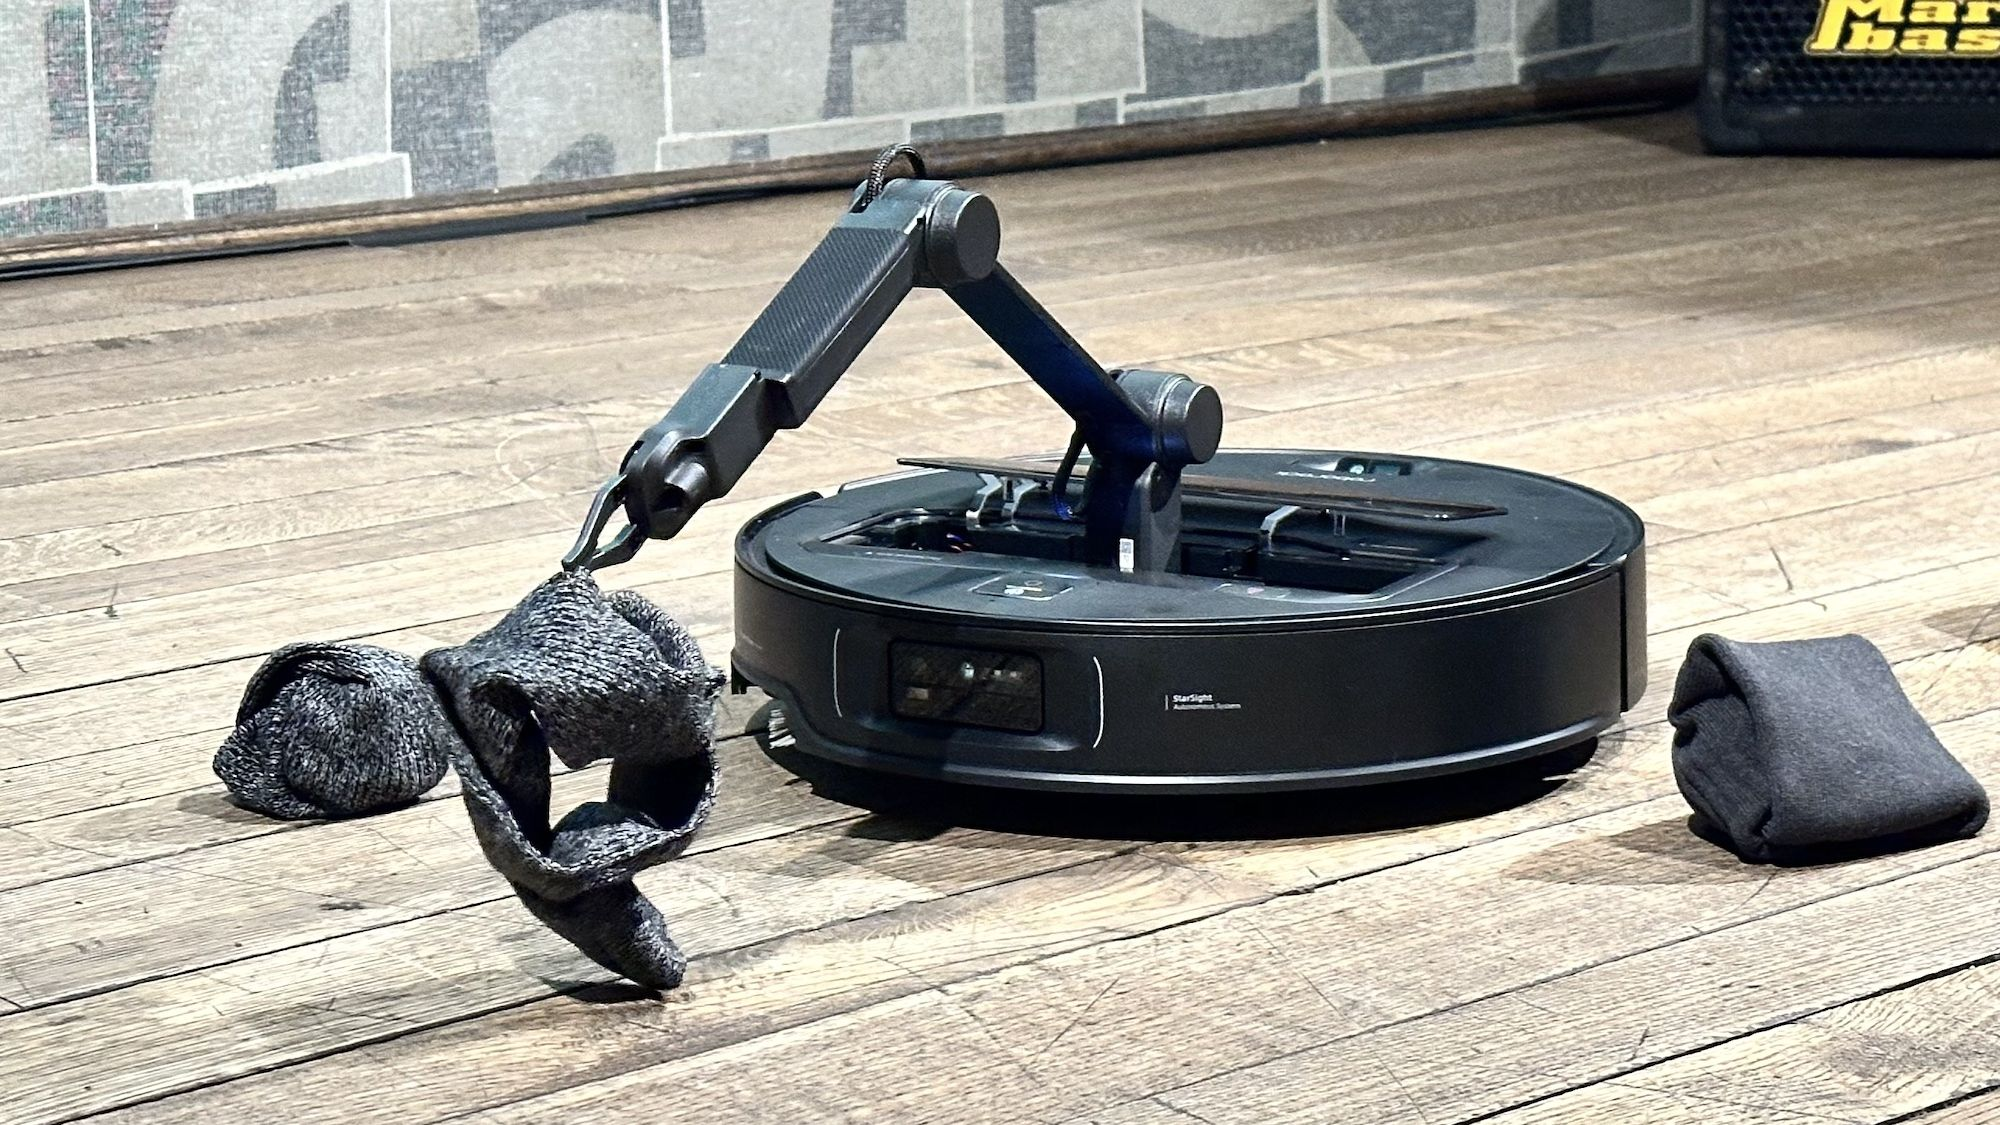
\includegraphics[width=0.6\textwidth]{figures/vacuum-cleaner.jpg}
\caption{Modern robotic vacuum cleaners utilize SLAM and localization technologies to autonomously navigate residential spaces, representing the most successful consumer robotics application to date.}
\label{fig:vacuum}
\end{figure}

The key to their success lies in the sophisticated implementation of SLAM (Simultaneous Localization and Mapping) and localization technologies. Modern robotic vacuum cleaners employ LiDAR sensors (Light Detection and Ranging), visual SLAM (VSLAM), and advanced mapping algorithms to create real-time maps of residential environments, enabling efficient path planning and obstacle avoidance \cite{neato2025}. This technology has proven so reliable that robotic vacuums have achieved nearly 40\% of the service robot market share \cite{trendforce2024}, demonstrating that autonomous navigation, when properly implemented, is mature enough for widespread consumer adoption.

    \item \textbf{Industrial Market: Amazon's Warehouse Robotics Dominance.}\newline
    In the industrial sector, the most successful large-scale application of AMRs (Autonomous Mobile Robots) has been warehouse automation, with Amazon leading the field. Amazon reports more than 750,000 to over one million robots across its fulfillment network, including drive units, mobile manipulators, and next-generation platforms such as Pegasus and Xanthus \cite{amazon2024ai, amazon2022}. These fleets demonstrate reliable fleet management, safe human–robot collaboration, and 24/7 uptime in highly dynamic environments.

\begin{figure}[H]
\centering
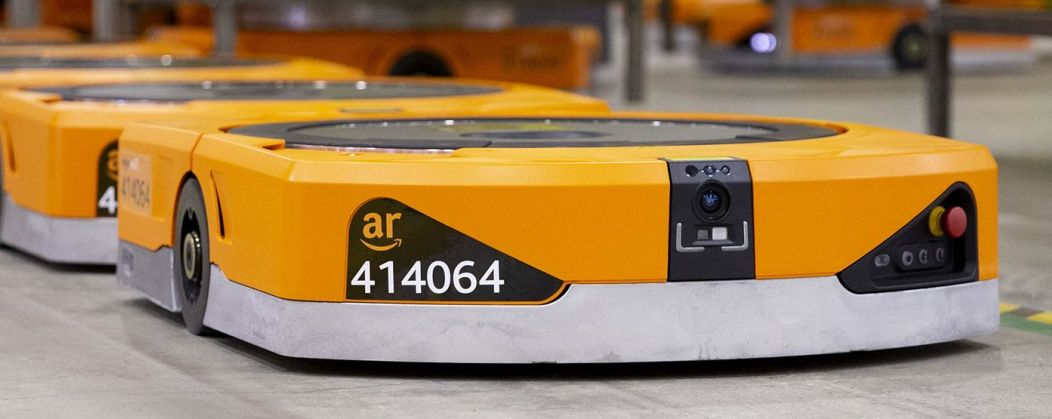
\includegraphics[width=0.9\textwidth]{figures/Amazon-Pegasus.jpg}
\caption{Amazon Pegasus drive unit used in high-throughput fulfillment centers.}
\label{fig:amazon-pegasus}
\end{figure}

    \item \textbf{Quadruped Robotics: Unitree Go2 as a Robust Mobility Platform.}\newline
    State-of-the-art quadruped robots such as Unitree Go2 demonstrate robust mobility on unpredictable terrain using reinforcement learning for locomotion policy optimization, advanced multi-sensor perception (3D LiDAR + depth/RGB cameras), and high-performance onboard compute for real-time planning and control. These capabilities enable operation on stairs, slopes, and uneven surfaces, with compelling applications in inspection, security, and emergency response \cite{unitreeGo2spec, unitreeRL2024}. Although not our primary target platform, Unitree’s capabilities illustrate complementary directions for rugged environments using RL and advanced multi-sensor perception, and inspire future extensions. 

\begin{figure}[H]
\centering
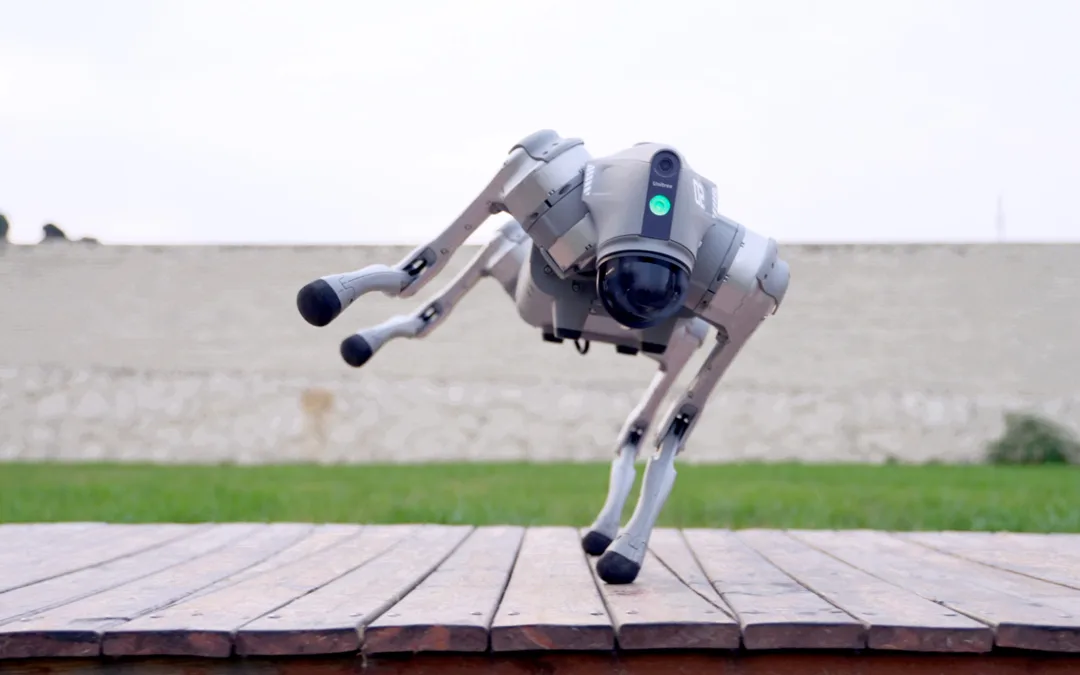
\includegraphics[width=0.9\textwidth]{figures/Unitree-Go2-6-copy-1080x675.png}
\caption{Unitree Go2: quadruped platform featuring RL locomotion, multi-sensor perception, and high-performance compute.}
\label{fig:unitree-go2}
\end{figure}
\end{enumerate}

\subsubsection{Benefits of Autonomous Mobile Robots in Healthcare Settings}

Recent literature and deployment data reveal multiple evidence-based benefits of AMRs in hospital environments:

\paragraph{Infection Control and Reduced Human Contact.}
AMRs significantly minimize human-to-human contact, reducing cross-contamination risks a critical advantage demonstrated during the COVID-19 pandemic \cite{intel2024, frontiers2024}. Autonomous delivery robots eliminate the need for multiple staff members to handle potentially contaminated materials, reducing occupational exposure and conserving personal protective equipment. UV-C (ultraviolet-C) disinfection robots have been shown to achieve 99.9\% pathogen kill rates on environmental surfaces, helping reduce hospital-acquired infections (HAIs) \cite{sciencedirect2021}.

\paragraph{Wayfinding and Visitor Guidance.}
Intelligent hospital guidance robots provide accurate navigation assistance to visitors and patients, reducing confusion and staff burden \cite{pmc2024nursing}. These robots can escort visitors to patient rooms, provide multilingual directions, and answer frequently asked questions about hospital facilities, allowing staff to focus on clinical care.

\paragraph{Material Transport and Delivery.}
AMRs excel at routine delivery tasks including medications, meals, linens, laboratory specimens, and medical supplies. This automation frees nursing staff from non-clinical transport duties, allowing them to spend more time on direct patient care. Studies indicate that delivery robots can reduce staff time spent on logistics by up to 30\% \cite{mdpi2024}.

\paragraph{Psychological Support and Patient Morale.}
Research consistently demonstrates that pediatric patients exhibit positive emotional responses to robot interactions \cite{beran2013}. Socially interactive robots reduce anxiety, provide distraction during painful procedures, and improve treatment compliance in children. Studies show that patients perceive robotic companions as non-judgemental, reducing psychological barriers to seeking help or expressing concerns \cite{ahu2024}.

\paragraph{Autonomous Disinfection and Cleaning.}
Cleaning and disinfection robots can be equipped with UV-C light systems at relatively low cost, providing continuous environmental sanitation \cite{intel2024}. These robots operate during off-peak hours without human supervision, ensuring consistent hygiene standards while minimizing disruption to clinical workflows.

\paragraph{Telepresence and Virtual Presence.}
AMRs with integrated telepresence capabilities enable remote consultations, family visits, and specialist rounds without requiring travel \cite{garingo2016}. This technology proved invaluable during pandemic restrictions and continues to provide value for rural healthcare access and specialist consultations.

\paragraph{Waste Collection and Handling.}
Some advanced AMR systems are deployed for biohazardous waste collection and disposal, reducing staff exposure to potentially infectious materials \cite{mdpi2024}. In China and other Asian markets, robots have been successfully implemented for collecting and transporting medical waste from patient rooms to centralized disposal areas, demonstrating significant improvements in operational efficiency and staff safety.

\subsubsection{Challenges in Hospital AMR Deployment}

Despite the significant benefits, several challenges remain:

\paragraph{Cost and Return on Investment.}
Hospital-grade AMRs represent substantial capital investments, typically ranging from \$50,000 to \$150,000 per unit depending on capabilities. Healthcare administrators require clear Return on Investment (ROI) demonstration through labor savings, efficiency gains, and improved outcomes to justify procurement \cite{mdpi2024}.

\paragraph{System Integration Complexity.}
Integrating AMRs with existing hospital information systems (HIS), electronic health records (EHR), elevator controls, automatic doors, and staff communication systems presents significant technical challenges. Interoperability standards are still evolving, requiring custom integration work for each deployment \cite{frontiers2024}.

\paragraph{Safety, Privacy, and Trust.}
Regulatory compliance (HIPAA, GDPR), patient data security, and physical safety in crowded environments remain critical concerns. Healthcare facilities must ensure that robots can safely navigate around patients, visitors, and medical equipment while maintaining patient privacy and data security \cite{jmir2024}. Building trust among staff and patients requires careful change management and demonstration of reliability.

\paragraph{Regulatory and Liability Issues.}
Medical device regulations, liability frameworks for autonomous systems, and insurance considerations create additional barriers to widespread adoption. Healthcare organizations must navigate complex approval processes and establish clear accountability frameworks for robot operations.

\subsubsection{Overview of Existing Robots in Healthcare}
The hospital robotics market has matured significantly, with several manufacturers deploying autonomous mobile robots at scale. Table~\ref{tab:competitive} presents a comprehensive comparison of leading hospital robot platforms currently deployed in eastern markets. Note that prices are approximate estimates and can vary significantly depending on region, configuration, volume, and additional features.

\begin{table}[H]
\centering
\small
\begin{tabular}{|l|p{2.5cm}|p{2cm}|p{1.5cm}|p{2.5cm}|p{4cm}|}
\hline
    \textbf{Rank} & \textbf{Manufacturer \& Model} & \textbf{Est. Deploy-ments} & \textbf{Est. Price (USD)} & \textbf{Key Hospital Applications} & \textbf{Features \& Notes} \\
\hline
1 & Pudu Robotics – PuduBot 2 \cite{pudubot2} & 15,000–20,000 units (~5,000 healthcare) & ~\$12,000 & Medication/meal delivery, linen transport, waste collection & Multi-floor navigation (elevator integration), VSLAM+LiDAR, 40 kg payload, 6–8 hr battery. Deployed in 100+ hospitals globally (China, Singapore, U.S.); customizable trays, infection-resistant coating. \\
\hline
2 & Keenon Robotics – M2 Medical Robot \cite{m2medical} & 8,000–10,000 units (healthcare-focused) & ~\$47,500 & UV-C disinfection, medication/lab sample delivery, patient room cleaning & UV sterilization (99.9\% pathogen kill rate), 40 kg payload, voice interaction, 10 hr runtime. Used in 100+ Chinese hospitals during COVID; exported to U.S./Europe (HIPAA-compliant). \\
\hline
3 & Pudu Robotics – PUDU CC1 \cite{puducc1} & 5,000–7,000 units (healthcare + hospitality) & ~\$16,800 & Floor cleaning, disinfection, material transport & Autonomous scrubbing (1,500 m²/hr), self-charging, obstacle avoidance. Popular in Chinese/U.S. hospitals for large-scale sanitation; integrates with PuduBot for hybrid tasks. \\
\hline
4 & Keenon Robotics – Peanut Medical \cite{peanutmedical} & 3,000–5,000 units & ~\$12,700 & Medication/meal delivery, patient guidance, telepresence & Compact (59 cm wide), multi-modal navigation, 30 kg payload. Deployed in Asia-Pacific hospitals; supports remote doctor-patient interaction via screen. \\
\hline
\end{tabular}
\caption{Competitive analysis of leading hospital AMR platforms by global deployment and capabilities.}
\label{tab:competitive}
\end{table}

\begin{figure}[H]
\centering
\begin{minipage}{0.45\textwidth}
\centering
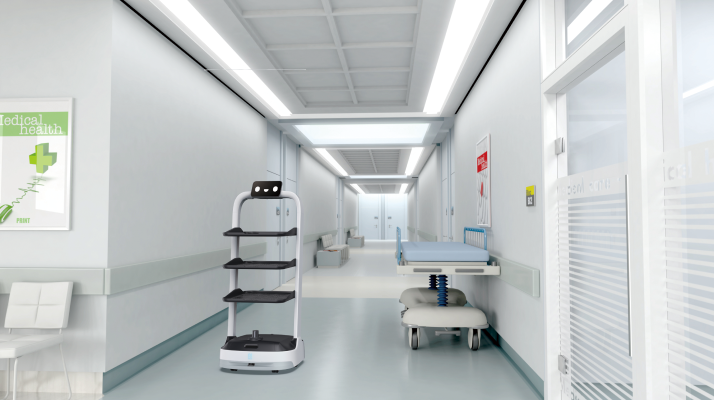
\includegraphics[width=\textwidth]{figures/pudubot-sante.png}
\caption{Pudu Robotics PuduBot 2}
\label{fig:pudubot}
\end{minipage}\hfill
\begin{minipage}{0.45\textwidth}
\centering
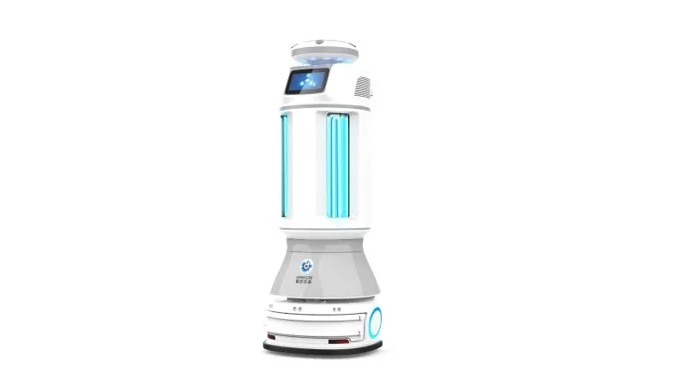
\includegraphics[width=\textwidth]{figures/KEENON-M2-Disinfection-Robot.jpg}
\caption{Keenon M2 Medical Robot}
\end{minipage}

\vspace{0.5cm}

\begin{minipage}{0.45\textwidth}
\centering
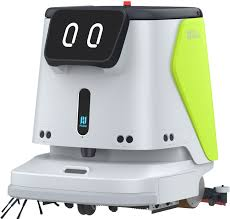
\includegraphics[width=\textwidth]{figures/pudu-cc1.jpeg}
\caption{Pudu Robotics PUDU CC1}
\label{fig:cc1}
\end{minipage}\hfill
\begin{minipage}{0.45\textwidth}
\centering
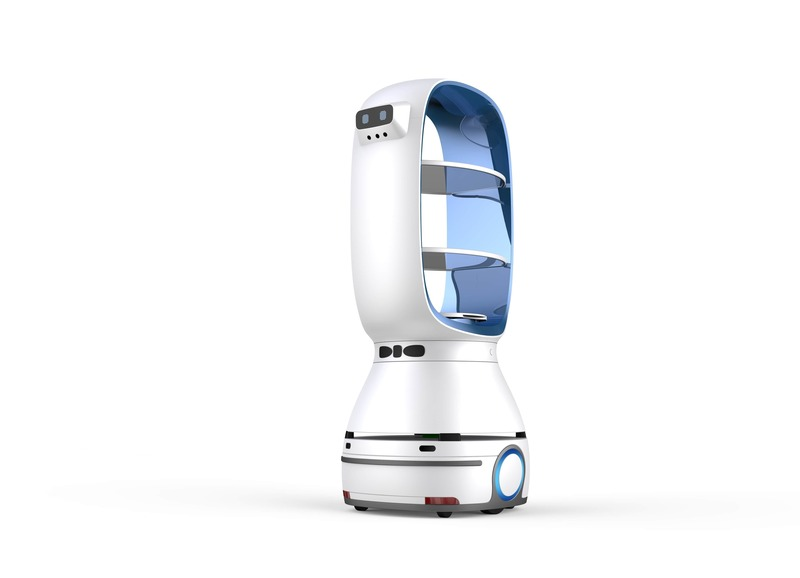
\includegraphics[width=\textwidth]{figures/peanut.jpg}
\caption{Keenon Peanut Medical}
\label{fig:peanut}
\end{minipage}
\end{figure}

In parallel, the field of Socially Assistive Robotics (SAR) has focused on the psycho-social aspects of patient care. These robots are designed not to perform physical tasks but to engage, encourage, and comfort patients through social interaction. For pediatric patients, robots like NAO and PARO (a therapeutic baby seal robot) have been shown to significantly reduce pain perception and anxiety during painful medical procedures such as vaccinations and chemotherapy \cite{beran2013}. The robot acts as a coach and a distractor, creating a more positive and cooperative atmosphere. For elderly populations, SARs have been explored for companionship to combat loneliness, provide cognitive stimulation for dementia patients, and deliver medication reminders to improve treatment adherence \cite{broekens2009}. These studies confirm that a robot's ability to interact socially is a powerful tool for improving patient well-being and clinical outcomes. The primary limitation of SARs, however, is that they are typically specialized, non-mobile or semi-autonomous platforms that lack the high-fidelity telepresence capabilities needed for direct clinical consultation.

\subsection{Technical Building Blocks}
This section deconstructs the essential technologies that form the foundation of an advanced autonomous healthcare robot. It examines navigation systems including Radio Frequency (RF) localization and SLAM-based sensor fusion, mobile robot platform specifications and selection criteria, Conversational AI and Large Language Models (LLMs) for intelligent interaction, and User Interface (UI) and Human-Robot Interaction (HRI) design paradigms for clinical integration.

\subsubsection{Navigation System}
The challenge of manual navigation highlighted in telepresence research is being addressed by autonomous mobile robots (AMRs). Modern AMRs employ a combination of SLAM, path planning, and obstacle avoidance to navigate complex environments without human intervention. The core navigation stack typically includes Radio Frequency (RF) Localization Technologies and SLAM-Based Sensor Fusion Techniques.

\paragraph{Radio Frequency (RF) Localization Technologies}
Radio frequency (RF) refers to electromagnetic waves (3 kHz--300 GHz) used for wireless communication. RF-based localization is essential where GPS is unreliable, such as indoors or through obstacles. Technologies like Wi-Fi, RFID, Bluetooth Low Energy (BLE), ZigBee, and Ultra-Wideband (UWB) are used, each selected based on coverage, scalability, battery life, accuracy, and cost. UWB, for example, enables multi-node scalability and multi-year tag battery life, but at higher cost (e.g., up to \$20,000 for a 5000~m$^2$ facility). Accuracy ranges from about 20~cm to over 1~m, with performance degrading in cluttered or metallic environments \cite{chen2022}. The general structure of these systems is to use static reference sensor locations, or anchors, within an environment, along with beacons or tags fixed to the objects with desired tracking. The location of the tracked object can be estimated using readings from the anchors. Mathematically, this estimation is commonly called multilateration (also called trilateration) when using distance measurements. Figure~\ref{fig:uwb} shows an example UWB anchor--tag geometry, while figure~\ref{fig:multilateration} illustrates the multilateration technique.
\begin{figure}[H]
\centering
\begin{minipage}{0.45\textwidth}
\centering
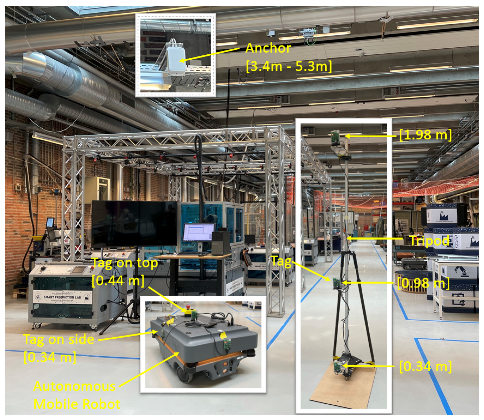
\includegraphics[width=\textwidth]{figures/uwb.png}
\caption{UWB anchor--tag geometry for ranging and multilateration-based localization in indoor environments.}
\label{fig:uwb}
\end{minipage}\hfill
\begin{minipage}{0.50\textwidth}
\centering
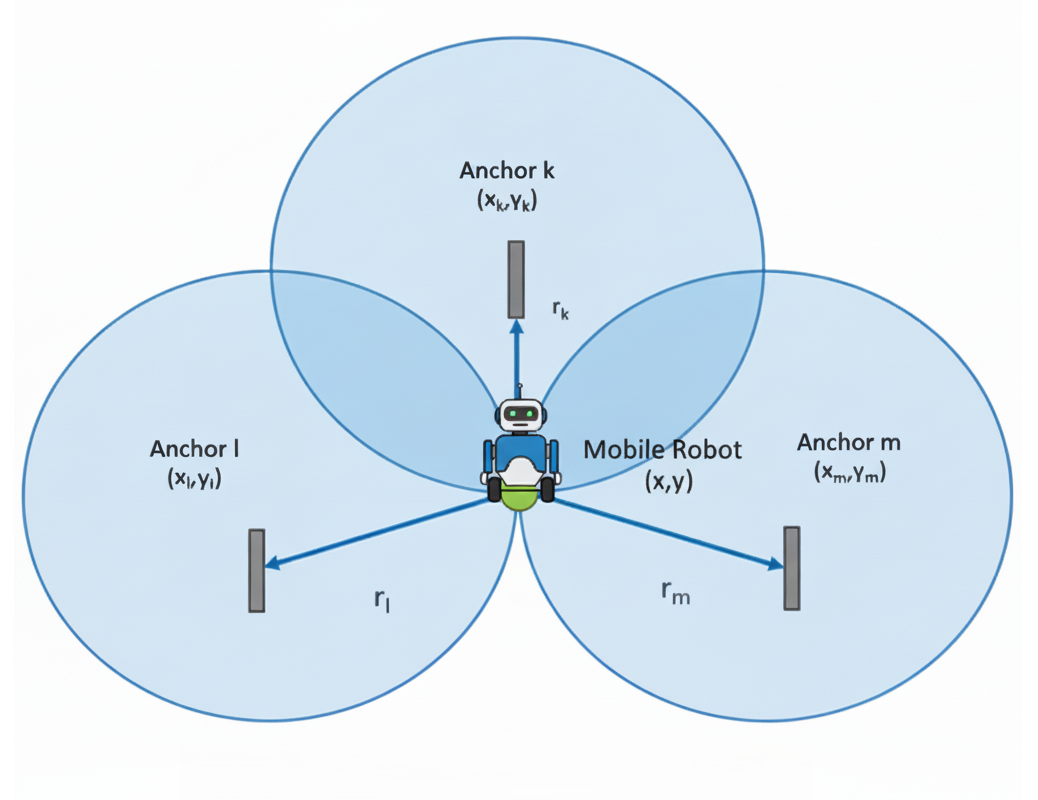
\includegraphics[width=\textwidth]{figures/Multilateration.png}
\caption{Illustration of multilateration technique. Each known anchor forms a circle with radius equal to its distance to the robot, and the robot’s estimated position is where these circles intersect.}
\label{fig:multilateration}
\end{minipage}
\end{figure}
Angle of Arrival (AoA) is a localization technique that determines the direction or angle from which a radio signal is received. An antenna array senses time differences across elements and applies signal-processing algorithms such as MUSIC or ESPRIT to convert those differences into an angle. AoA (often via BLE 5.1+ or UWB Direction Finding) estimates a target's angle using a beacon or tag and a robot-mounted antenna array, reducing reliance on dense static infrastructure. BLE-based tags offer excellent battery life (years). Limitations include line-of-sight sensitivity and variable accuracy; hybrid AoA + RSSI filtering can improve precision, achieving mean errors on the order of 12 cm in simulation even in cluttered settings \cite{weinmann2023}. AoA could be used to implement a solution that does not depend on localization or positioning infrastructure in the environment, instead having the robot home in on a beacon worn by the user. This would be similar to how some Bluetooth trackers work for finding lost items. The robot would use the angle of arrival data to determine the direction to move towards the beacon signal, allowing it to autonomously navigate to the user's location. This approach could be particularly useful in dynamic environments like hospitals where fixed infrastructure may not be feasible. Figure~\ref{fig:amr-stack} illustrates a proposed setup where a Bluetooth homing controller on the robot uses AoA data from a wearable beacon to guide navigation towards the target. Multiple anchors could be used to implement waypoints following navigation paths through the environment. 

\begin{figure}[H]
\centering
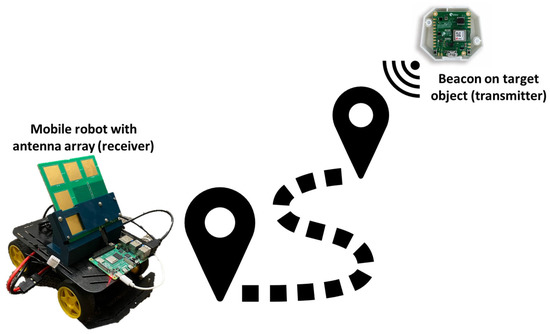
\includegraphics[width=0.5\textwidth]{figures/config.jpg}
\caption{Configuration of proposed setup of Bluetooth homing controller.}
\label{fig:amr-stack}
\end{figure}

\paragraph{SLAM-Based Sensor Fusion Techniques}
Simultaneous Localization and Mapping (SLAM) is a critical technology for autonomous navigation, enabling robots to build maps of unknown environments while simultaneously keeping track of their own location. Its effectiveness hinges on robust sensor fusion techniques that integrate data from various sources such as camera(s), IMU, wheel odometry, or RF ranging. Beyond external RF systems, autonomous navigation heavily relies on SLAM with multi-sensor fusion for robustness. A common stack fuses 2D LiDAR with an IMU and wheel odometry. IMU and odometry constrain motion, correcting LiDAR motion distortion and mitigating slip-induced drift. Studies report substantial gains when integrating IMU and wheel odometry, for example, approximately 27\% improvement in rotation error and greater than 67\% reduction in position error relative to LiDAR only SLAM, at the expense of added system complexity and compute \cite{doduc2024}.

VSLAM (Visual Simultaneous Localization and Mapping) is a method that uses cameras to help robots figure out where they are and build maps of their surroundings at the same time. VSLAM uses cameras like monocular (single), stereo (two), or RGB-D (depth-sensing) for positioning and mapping. It provides low-cost, lightweight hardware and better scene understanding. Challenges include poor performance in texture-less or repetitive areas, and scale issues in monocular systems (e.g., early ORB-SLAM 2.0). Modern approaches prefer hybrid Visual–Inertial–Ranging–LiDAR (VIRAL) SLAM for improved reliability in complex environments \cite{tourani2022}. Figure~\ref{fig:slam} shows the combination of visual/laser data with inertial and odometric inputs for stable estimation. Tools like Google Cartographer build 3D maps in real-time, using LiDAR, IMU, and odometry. 
\begin{figure}[H]
\centering
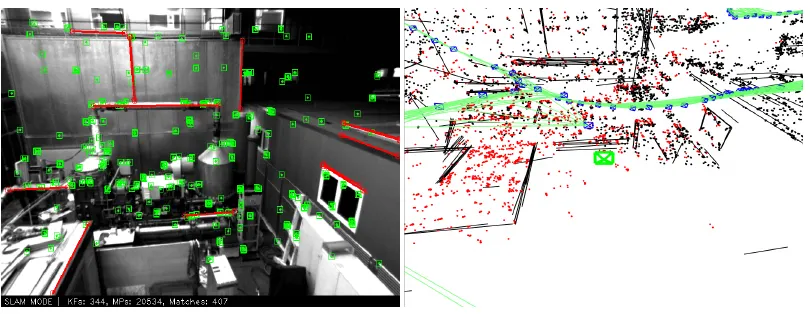
\includegraphics[width=0.75\textwidth]{figures/slam.png}
\caption{Illustration of SLAM fusion: visual/laser perception integrated with inertial and odometric constraints for robust state estimation.}
\label{fig:slam}
\end{figure}

\paragraph{Navigation Systems Across Hospital Robotics Platforms.}
Table~\ref{tab:robot_nav} summarizes the navigation technologies and sensor configurations employed by leading hospital robotics platforms mentioned in table \ref{tab:competitive}.

\begin{table}[H]
\centering
\small
\begin{tabular}{|l|p{2.5cm}|p{2.5cm}|p{3.5cm}|}
\hline
\textbf{Robot Model} & \textbf{Primary Localization} & \textbf{Mapping Technology} & \textbf{Key Sensors} \\
\hline
PuduBot 2 \cite{pudubot2} & SLAM (LiDAR-based) & Real-time 2D/3D mapping & 2D LiDAR, depth camera, IMU \\
\hline
M2 Medical Robot \cite{m2medical} & SLAM (LiDAR-based) & Real-time 2D mapping & 2D LiDAR, RGB camera, encoders \\
\hline
PUDU CC1 \cite{puducc1} & SLAM (LiDAR-based) & Real-time 2D mapping & 2D LiDAR, ultrasonic sensors, encoders \\
\hline
Peanut Medical \cite{peanutmedical} & Hybrid (SLAM + RF) & Real-time 2D mapping & LiDAR, depth sensors, optional UWB \\
\hline
\end{tabular}
\caption{Navigation systems and sensor technologies across leading hospital robotics platforms.}
\label{tab:robot_nav}
\end{table}

\subsubsection{Mobile Robot Platform specifications}

The selection of an appropriate mobile robot platform is a critical decision that directly impacts system reliability, development time, and operational costs. For a healthcare telepresence robot operating in hospital corridors and patient rooms, the platform must satisfy several essential technical and operational requirements while remaining within practical budget constraints.

\paragraph{Platform Requirements.}
The system requires a wheeled mobile robot platform with the following capabilities:

\begin{itemize}[leftmargin=*]
    \item \textbf{Autonomous docking and charging} with high-level API commands (\texttt{dock()}, \texttt{return\_to\_charge()})
    \item \textbf{ROS/ROS 2 compatibility} for navigation packages (Nav2, SLAM Toolbox, AMCL)
    \item \textbf{Payload capacity} of 5--10~kg for telepresence screen, onboard computer, and camera system
    \item \textbf{Indoor navigation sensors} including LiDAR (2D or 3D) and depth cameras
    \item \textbf{Safety and reliability} features (cliff detection, bumpers, emergency stop)
\end{itemize}

\paragraph{Project Constraints.}
Budget constraints significantly influence platform selection. The target budget for the mobile base, charging dock, and core sensors is approximately \$1,000--\$1,500 USD, recognizing that higher-cost industrial platforms (\$5,000+) exceed the scope of an educational research project. Additional constraints include global availability (shipping to Oman), vendor support and documentation quality, and community resources for troubleshooting and development.

\paragraph{Platform Comparison.}
Table~\ref{tab:platforms} presents a comparative analysis of commercially available mobile robot platforms. 

\begin{table}[H]
\centering
\footnotesize
\begin{tabular}{|p{3.2cm}|l|c|c|c|p{4.5cm}|}
\hline
\textbf{Platform} & \textbf{Price (USD)} & \textbf{Dock} & \textbf{ROS} & \textbf{Payload} & \textbf{Notes} \\
\hline
\multicolumn{6}{|c|}{\textit{Budget Tier (\$500--\$1,000)}} \\
\hline
iRobot Create 3 \cite{irobot2024create3} & \$549 & Yes & ROS 2 & 9~kg & Roomba-based, proven docking, ideal for education \\
\hline
Yahboom ROSMASTER X3 \cite{yahboom2024} & \$699 & DIY & ROS 1 & 5--8~kg & Mecanum wheels, requires custom docking solution \\
\hline
Elephant Robotics MyAGV 2023 \cite{elephantrobotics2024} & \$899 & DIY & ROS 1 & 8~kg & Mecanum wheels, 2D SLAM ready, Python/ROS compatible \\
\hline
\multicolumn{6}{|c|}{\textit{Mid-Tier (\$1,000--\$2,000)}} \\
\hline
SLAMTEC Apollo \cite{slamtec2024} & \$1,200 & Yes & ROS 1/2 & 50~kg & Same platform as Pudu/Keenon hospital robots \\
\hline
TurtleBot 4 Standard \cite{turtlebot2024} & \$1,400 & Yes & ROS 2 & 9~kg & Research-grade, Nav2 pre-configured, Lidar included \\
\hline
Husarion ROSbot 2R \cite{husarion2024} & \$1,600 & Optional & ROS 2 & 10~kg & Mecanum wheels, hospital navigation demos available \\
\hline
AgileX LIMO Pro \cite{agilex2024} & \$1,799 & Optional & ROS 2 & 10~kg & 4-mode steering, Jetson Nano, research platform \\
\hline
\end{tabular}
\caption{Comparative analysis of mobile robot platforms for healthcare telepresence applications.}
\label{tab:platforms}
\end{table}


\subsubsection{Conversational AI and Large Language Models (LLMs)}
\label{sec:llm}
The field of large language models (LLMs) has witnessed transformative advancements, establishing them as a core technology for conversational AI. An LLM is a sophisticated artificial intelligence system trained on vast datasets of text and code, enabling it to understand, generate, and interact with human language in a nuanced manner. These models have rapidly transitioned from research prototypes to industrial-scale technologies, resulting in a proliferation of models with distinct strengths and commercial terms.

The LLM landscape is broadly divided into two categories: open-source and proprietary. Open-source models, such as Meta's Llama series and the DeepSeek series, offer significant flexibility, allowing for deep customization and fine-tuning to meet specific application needs, often at a lower cost \cite{civo2024}. However, they may require more complex setup and can sometimes lag behind proprietary counterparts in raw performance. In contrast, privately-owned models like OpenAI's GPT series and Google's Gemini series typically offer state-of-the-art performance and are adept at handling highly complex tasks. This performance comes with trade-offs, including higher operational costs and potential data privacy concerns, which are critical considerations in healthcare applications \cite{musick2025}. The selection of an LLM depends on a careful balance between performance requirements, budget, customizability, and data governance policies. Table~\ref{tab:llm_comparison} provides a comparative overview of leading LLM options.

\begin{table}[H]
\centering
\small
% Use tabularx to make the table fit the text width. X columns will wrap text.
% The >{\...} commands are for text alignment within the columns.
\begin{tabularx}{\textwidth}{| >{\raggedright\arraybackslash}X | l | >{\raggedright\arraybackslash}X | >{\centering\arraybackslash}X | >{\centering\arraybackslash}X | >{\centering\arraybackslash}X |}
\hline
\textbf{Model (Version)} & \textbf{Org.} & \textbf{License} & \textbf{Max Context (tokens)} & \textbf{Input API Cost (\$/M)} & \textbf{Output API Cost (\$/M)} \\
\hline
OpenAI GPT-5.2 \cite{openai2025pricing} & OpenAI & Proprietary & 128,000 & \$1.75 & \$14.00 \\
\hline
Google Gemini 3 Flash \cite{google2025pricing} & Google & Proprietary & 1,000,000 & \$0.50 & \$3.00 \\
\hline
Google Gemini 2.5 Pro \cite{google2025pricing} & Google & Proprietary & 1,000,000 & \$1.25--\$2.50 & \$10.00--\$15.00 \\
\hline
Google Med-Gemma 2B & Google & Open Weight (Apache 2.0) & 8,192 & \$0.00 (Self-hosted) & \$0.00 (Self-hosted) \\
\hline
Meta Llama 4 Maverick \cite{llama2025} & Meta & Llama Community License & 10,000,000 & \$0.19--\$0.49 & \$0.19--\$0.49 \\
\hline
DeepSeek V3.1 \cite{deepseek2025} & DeepSeek & MIT (Code) / DeepSeek Model & 128,000 & \$0.14 & \$0.28 \\
\hline
\end{tabularx}
\caption{Comparative analysis of leading Large Language Models with December 2025 pricing and specifications.}
\label{tab:llm_comparison}
\end{table}

\paragraph{LLM Discussion and Cost Considerations.}
Table~\ref{tab:llm_comparison} summarizes key characteristics of leading LLM options as of December 2025. OpenAI's GPT-5.2 offers strong performance with a 128k token context window at \$1.75/\$14.00 per million input/output tokens. Google's Gemini 3 Flash provides exceptional value with a 1M token context and competitive pricing at \$0.50/\$3.00, with free tier available for development (up to 500 requests per day). Google's Gemini 2.5 Pro offers higher capabilities for complex tasks at \$1.25--\$2.50 input and \$10.00--\$15.00 output per million tokens. Google's Med-Gemma represents a family of specialized open-weight models (available in 2B, 7B, and 27B parameter variants) fine-tuned specifically on medical literature, clinical guidelines, and healthcare datasets \cite{medgemini2024}. While Med-Gemma demonstrates state-of-the-art performance on medical benchmarks (MedQA, MedMCQA, PubMedQA) and would be highly relevant for advanced clinical decision support or medical question answering, it is considered overkill for the basic conversational interactions required in this project (patient guidance, wayfinding, simple information queries). Meta's Llama 4 Maverick stands out with an unprecedented 10M token context window and industry-leading cost efficiency (\$0.19--\$0.49 per million tokens), making it highly suitable for long-context healthcare applications. DeepSeek V3.1 offers the most economical option at \$0.14/\$0.28 per million tokens, particularly beneficial for cost-sensitive deployments. For this project's conversational requirements (patient guidance, wayfinding, simple information queries), either Gemini 3 Flash (free tier) or DeepSeek V3.1 (lowest cost) would be appropriate choices, with Llama 4 Maverick offering future-proof long-context capabilities if advanced document processing becomes necessary.

\subsubsection{User Interface and Human-Robot Interaction}
For autonomous healthcare robots operating in clinical environments, the user interface (UI) and human-robot interaction (HRI) design directly impacts adoption, user satisfaction, and clinical workflow integration. The interface must balance accessibility for diverse user groups (clinicians, administrative staff, patients) with robust control mechanisms suitable for dynamic hospital environments. Common UI paradigms employed in hospital robotics include:

\paragraph{Onboard Touchscreen Interface.}
A dedicated touchscreen mounted on the robot body provides direct, localized control and real-time status feedback. Common in systems like Pudu Robotics' PuduBot 2 and Keenon Robotics' M2 Medical Robot, these interfaces typically run Android OS and display navigation status, task queues, and emergency controls. Advantages include intuitive interaction without external devices and immediate feedback. Limitations include reliance on the robot's physical proximity and potential hygiene concerns in sterile environments \cite{m2medical}.

\paragraph{Mobile Application (iOS/Android).}
Native mobile applications running on clinicians' and administrators' smartphones or tablets enable remote operation and fleet monitoring from anywhere within hospital networks. This approach is ubiquitous across commercial systems (PuduBot 2, M2, Peanut Medical) and supports features such as route customization, real-time tracking, task scheduling, and status notifications. Mobile apps offer flexibility and integrate seamlessly with existing hospital workflows, though they require network connectivity and depend on user device management \cite{pudubot2}.

\paragraph{Web-Based Dashboard.}
Cloud-hosted or on-premises web portals provide centralized fleet management, historical analytics, and administrative controls for hospital operators and IT administrators. Systems like Keenon Robotics and Pudu Robotics include web dashboards for route optimization, performance metrics, and multi-robot coordination. Web interfaces support remote monitoring across multiple locations and facilitate integration with hospital information systems (HIS). Trade-offs include network dependency, data security considerations, and potential latency in real-time control \cite{puducc1}.

\paragraph{Voice Control and Natural Language Interfaces.}
Voice-based interaction leveraging conversational AI and LLMs (as discussed in Section~\ref{sec:llm}) represents an emerging paradigm for hands-free operation in clinical settings. Systems like Keenon's M2 support voice commands, allowing clinicians to interact with robots while maintaining hygiene and workflow continuity. Voice interfaces reduce cognitive load and support more natural, intuitive interactions, but require robust speech recognition, noise handling (hospital environments are loud), and contextual understanding \cite{musick2025}.

\paragraph{Hospital Integration via APIs.}
Integration with existing hospital IT infrastructure through RESTful APIs or DICOM/HL7 standards allows robots to receive task assignments directly from electronic health records (EHR) or hospital management systems. This approach minimizes manual input and ensures tasks are coordinated with clinical workflows. Examples include systems capable of receiving delivery requests directly from hospital pharmacies or labs \cite{puducc1}.

\paragraph{Robot UI Usage Across Hospital Platforms.}
Table~\ref{tab:robot_ui} summarizes the UI and interaction modalities employed by leading hospital robotics platforms, illustrating the diversity of approaches and trade-offs in current systems.

\begin{table}[H]
\centering
\small
\begin{tabular}{|l|p{2cm}|p{2.5cm}|p{2.5cm}|p{2.5cm}|}
\hline
\textbf{Robot Model} & \textbf{Onboard Screen} & \textbf{Mobile App} & \textbf{Web Dashboard} & \textbf{Voice/AI Interface} \\
\hline
PuduBot 2 \cite{pudubot2} & Android tablet & iOS/Android & Yes & Limited \\
\hline
M2 Medical Robot \cite{m2medical} & Android display & iOS/Android & Yes & Yes (voice control) \\
\hline
PUDU CC1 \cite{puducc1} & Android panel & iOS/Android & Yes & No \\
\hline
Peanut Medical \cite{peanutmedical} & Optional & iOS/Android & Yes & Limited \\
\hline
\end{tabular}
\caption{UI and interaction modalities across leading hospital robotics platforms.}
\label{tab:robot_ui}
\end{table}

\clearpage

\subsection{Conclusion}

The literature presents a clear picture:
\begin{enumerate}
    \item \textbf{Telepresence robots} are effective for remote diagnosis but are limited by manual control and an impersonal user experience.
    \item \textbf{Socially assistive robots} have proven their value in patient engagement and comfort but lack clinical telepresence and advanced mobility.
    \item \textbf{Autonomous mobile robots} have mastered navigation in hospitals but are used for logistics, not patient interaction.
    \item \textbf{Conversational AI} offers intelligent dialogue but lacks the physical embodiment needed for meaningful healthcare encounters.
    \item \textbf{Consumer and industrial robotics} have demonstrated that autonomous navigation technology is mature, reliable, and cost-effective for real-world deployment, as evidenced by millions of robotic vacuum cleaners in homes and over one million AMRs in Amazon warehouses.
    \item \textbf{Current hospital AMRs} are predominantly focused on material transport and disinfection, with limited integration of social interaction, advanced telepresence, and conversational AI capabilities.
\end{enumerate}

The critical research gap lies at the intersection of these domains. There is a demonstrable need for a single, integrated platform that combines the \textbf{clinical access} of a telepresence robot, the \textbf{patient-centric engagement} of a SAR, the \textbf{operational independence} of an autonomous navigator, and the \textbf{interactive intelligence} of modern conversational AI. The proven success of autonomous navigation in consumer (robotic vacuums) and industrial (Amazon warehouses) applications demonstrates that the core technology is mature and ready for advanced healthcare applications.

This project directly addresses this gap by designing a holistic system that synthesizes these strengths, creating a smart healthcare robot capable of not only connecting doctors and patients but also navigating its environment independently and engaging with patients in a helpful and empathetic manner. By learning from the successes of consumer robotics, warehouse automation, and existing hospital AMR deployments, this project aims to advance the state-of-the-art in healthcare robotics toward truly integrated, intelligent, and patient-centered care.

\clearpage
